\section{Effets :}
\emph{Interface :}

L'utilisateur choisit un effet parmi la liste d'effets affichée en bas de l'écran. Il a ensuite accès aux 
réglages disponibles, s'il y en a. L'utilisateur peut ensuite choisir de confirmer ou d'annuler la modification
apportée par l'effet choisi.
\\

\emph{Structure du code :}

Les effets sont rassemblés dans le package filters (fr.ubordeaux.pimp.filters).
La classe \emph{Retouching} contient les réglages de luminosité, contraste, saturation et teinte.
La classe \emph{Convolution} contient tous les effets liés à la convolution (flou, détection de contour etc.).
Toutes ces méthodes sont appelées lors de l'appui de boutons ou de glissement de seekbars.
\subsection{Luminosité (Brightness) :}
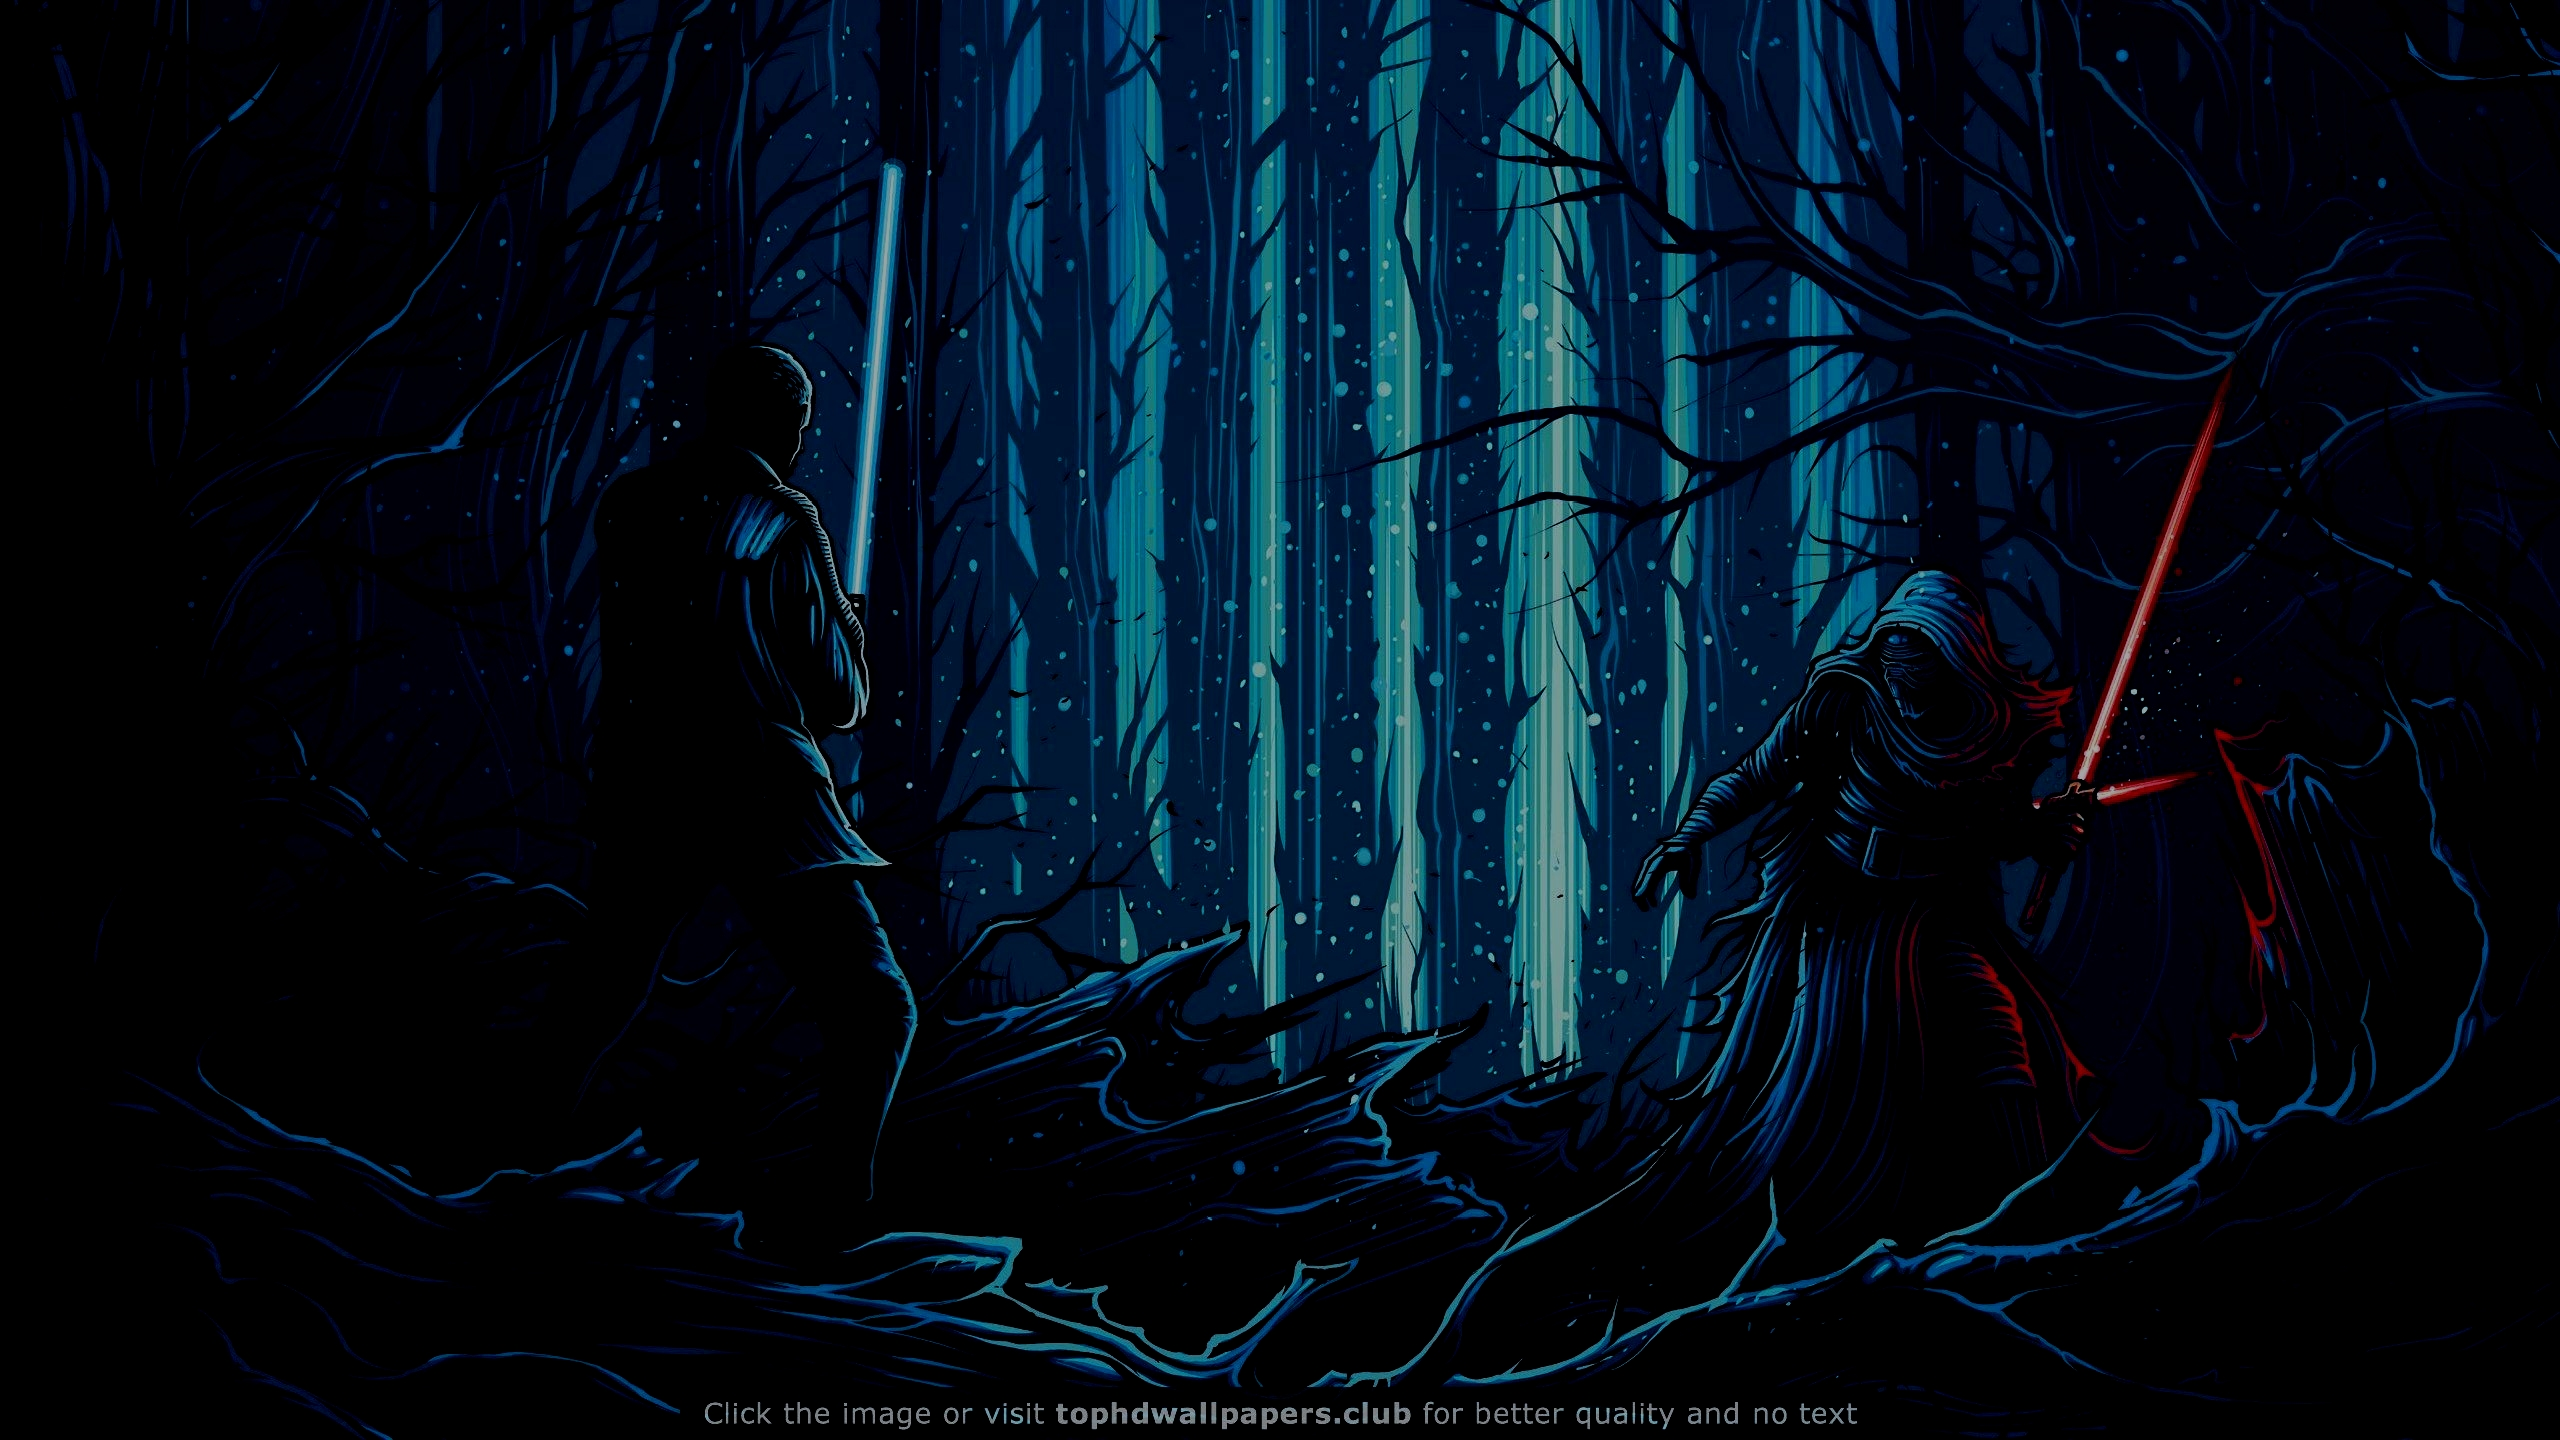
\includegraphics[width=0.5\textwidth]{report_src/brightness_low.jpeg}
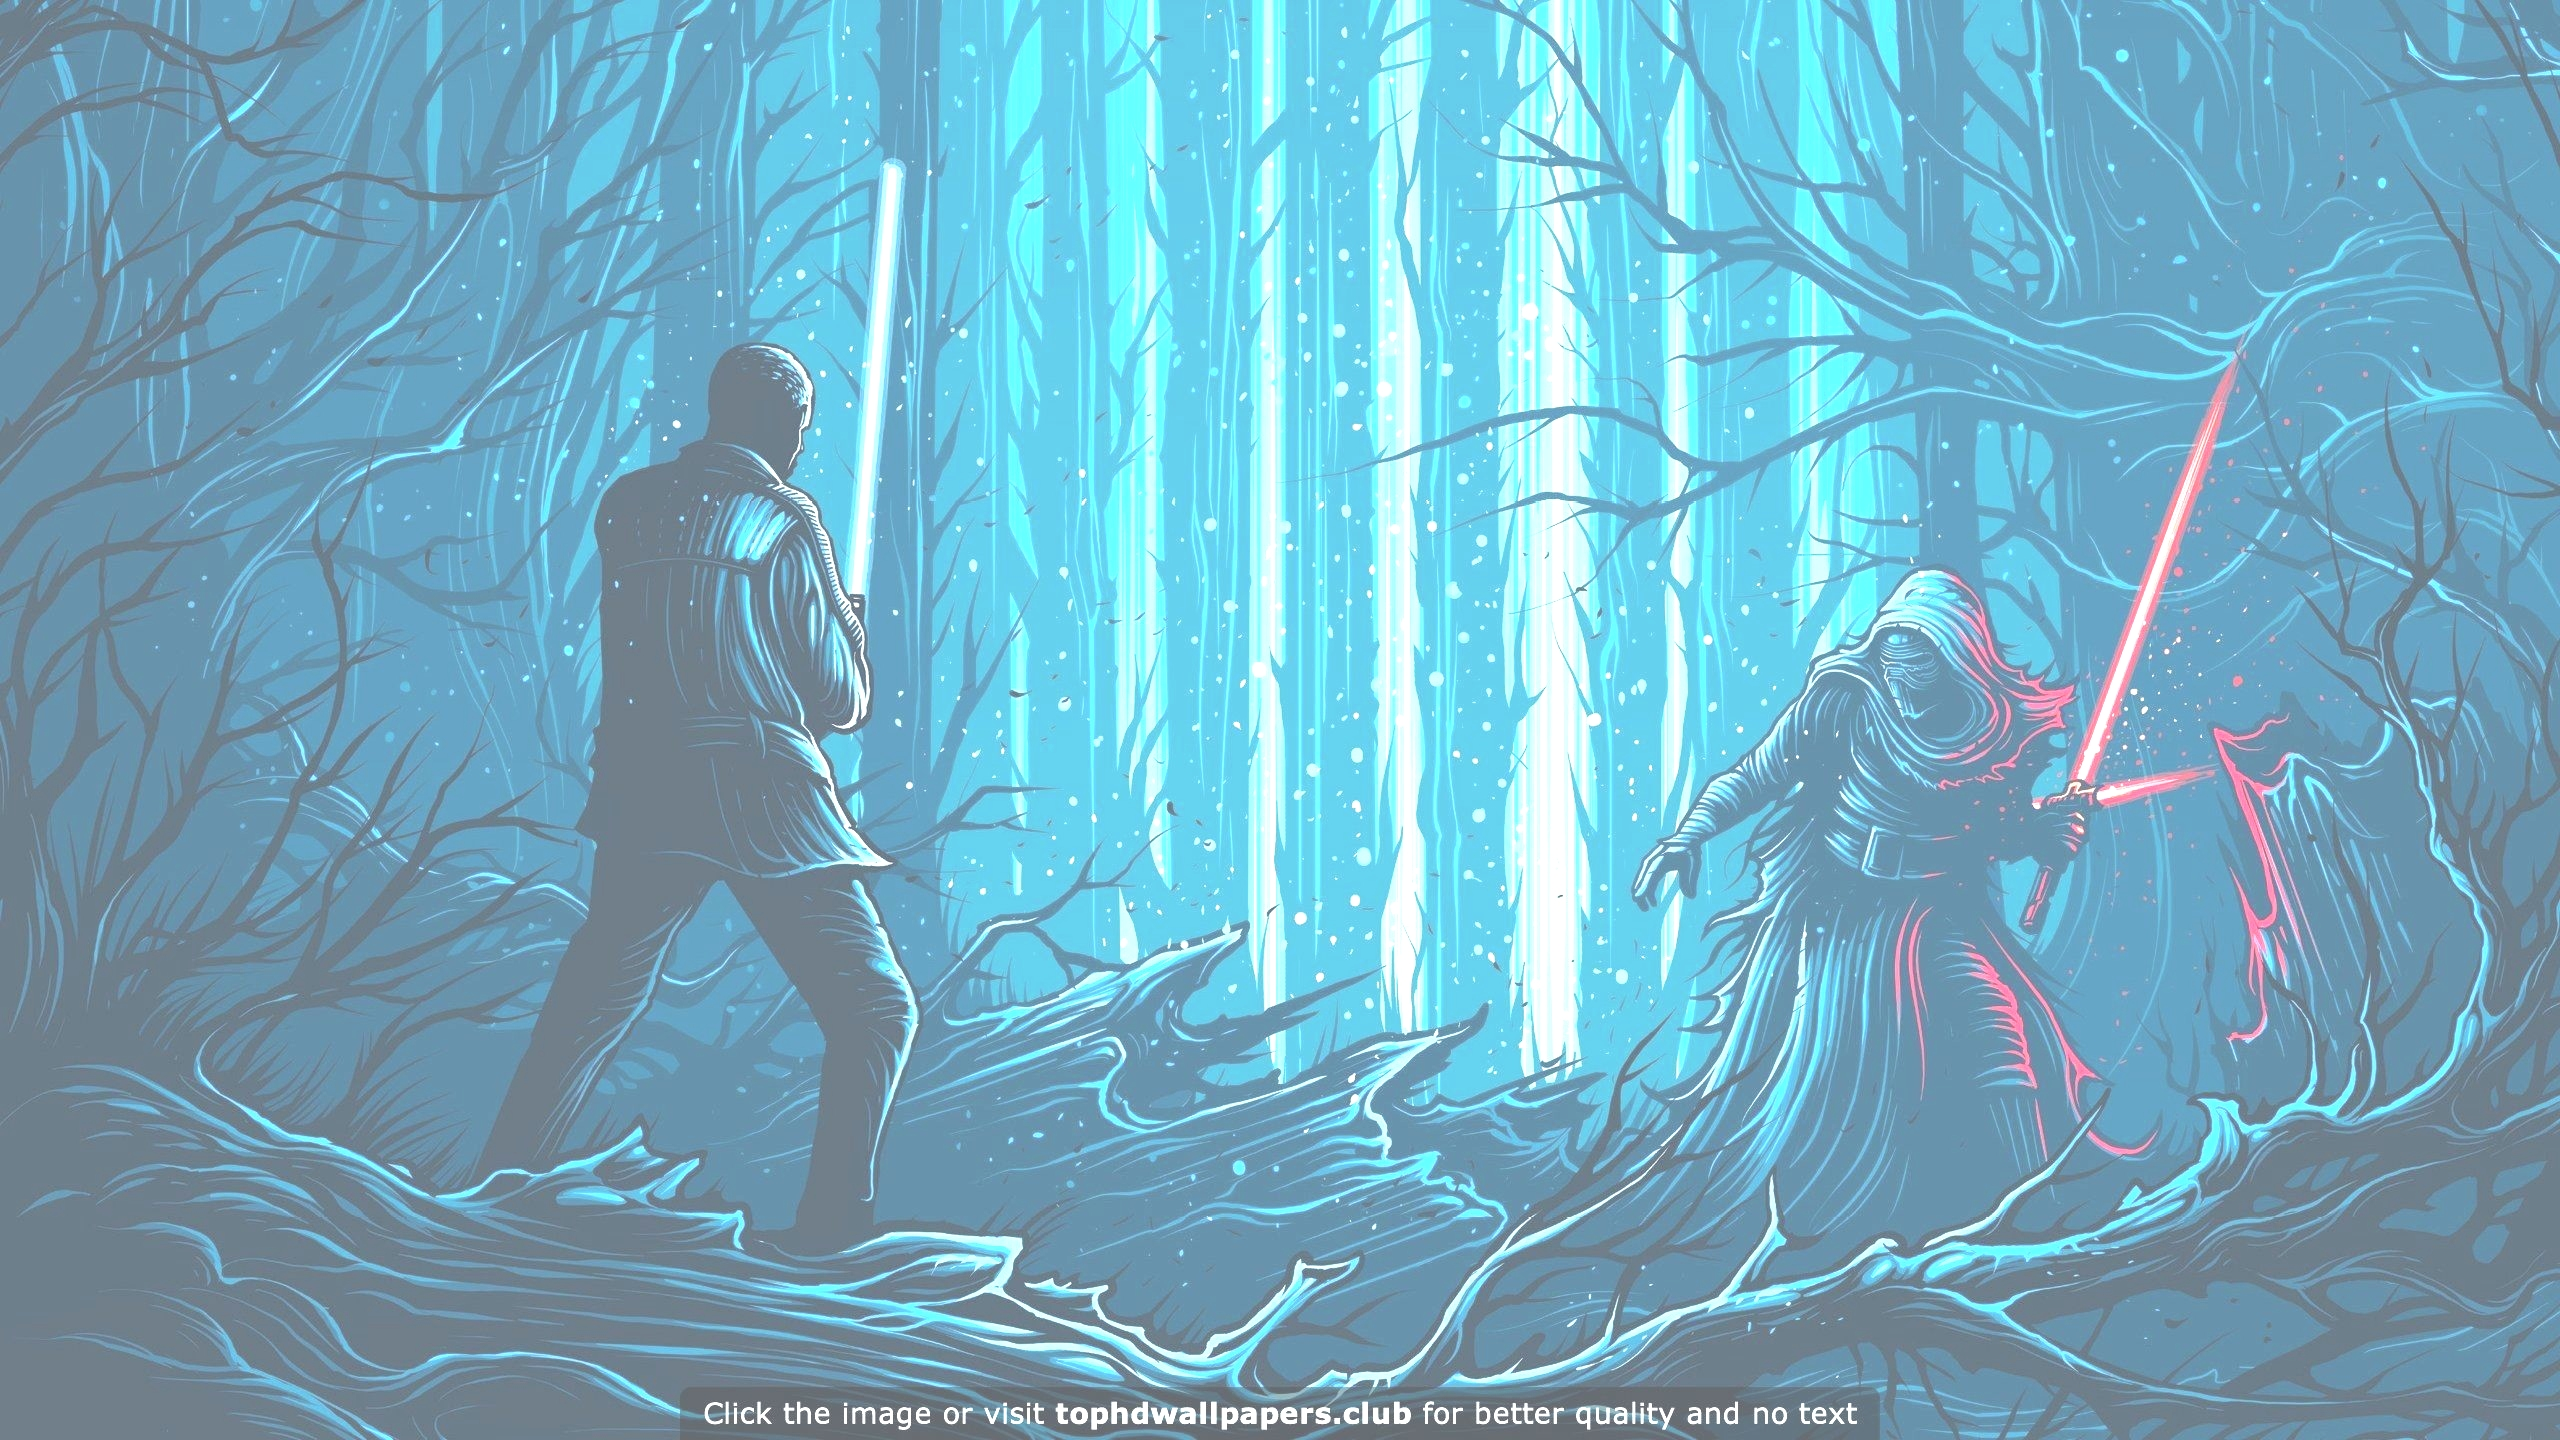
\includegraphics[width=0.5\textwidth]{report_src/brightness_high.jpeg}

\subsection{Contraste (Contrast) :}
\subsection{Saturation (Saturation) :}